\documentclass[10pt, oneside,spanish]{article}   	
\usepackage{geometry}
\usepackage{amsmath}
\geometry{a4paper}                   		
\usepackage[utf8]{inputenc}               	 
\usepackage{listings}	
\usepackage{tabu}


\usepackage{graphicx}												
\usepackage{amssymb}
\usepackage{authblk}
\usepackage{relsize}



\linespread{1.5}

\title{MKTG 212 - Case 4: Logistic Regression \& Clustering Methods} \lstset{language=R}

\author[]{Juan Manubens}

\affil[]{University of Pennsylvania}
\renewcommand\Authands{, }
\date{}							
\begin{document}
\maketitle







\section{Brand Awareness}

\textit{There is a lot of interest in how TV viewing (and other demographics) relates to awareness of new brands. A new detergent brand CSG collected some data on households. The data is available on Canvas (Assignments / Assignment4 / Tv\_viewing.txt).  The variables in the dataset for a random sample of 500 households are as follows:}\\

\begin{center}
\begin{tabular}{ | c | c |  }
 \hline
\textbf{Variable Name} & \textbf{Description}  \\
 \hline
 HH Number: & Household ID  \\
 \hline
Hours TV: & \# Hours of TV Viewing per week \\ 
 \hline
DeterPur: & \# of detergent purchases in the last calendar year
  \\
  \hline
Gender: & Gender of Head of Household (1=Male, 0=Female)  \\
  \hline
Income: & Household Income in thousands of dollars  \\
  \hline
Aware CSG: & Awareness or not of new Brand CSG (1 = aware of CSG, 0 otherwise)
  \\
  \hline
\end{tabular}
\end{center}
\medskip

\pagebreak

\begin{itemize}
\item \textbf{[1a] Which of the variables is the most significant \textit{single predictor} (i.e. one variable at a time) of AwareCSG, awareness or not of CSG?  State how you arrived at this conclusion?  Is it a significant predictor at the 1\% significance level?  }
\end{itemize}

\textbf{Run an appropriate regression with dependent variable = aware CSG and independent variables = Hours TV, DeterPur, Gender and Income.  Based on this regression, answer the following questions}

%q1i.col2 <- glm(AwareCSG ~  HoursTV, family = binomial(link = "logit"), data = views)
%q1i.col2.summary <- summary(q1i.col2); q1i.col2.summary$coefficients
%#               Estimate Std. Error   z value     Pr(>|z|)
%#(Intercept) -1.78006428 0.32995509 -5.394868 6.857378e-08
%#HoursTV      0.08212197 0.01466808  5.598686 2.159822e-08

%q1i.col3 <- glm(AwareCSG ~  DetergentPur, family = binomial(link = "logit"), data = views)
%q1i.col3.summary <- summary(q1i.col3); q1i.col3.summary$coefficients
%#                Estimate Std. Error    z value  Pr(>|z|)
%#(Intercept)  -0.08413269 0.17509974 -0.4804844 0.6308830
%#DetergentPur  0.02719424 0.04865845  0.5588802 0.5762435

%q1i.col4 <- glm(AwareCSG ~  as.factor(Gender), family = binomial(link = "logit"), data = views)
%q1i.col4.summary <- summary(q1i.col4); q1i.col4.summary$coefficients
%#                        Estimate Std. Error       z value Pr(>|z|)
%#(Intercept)        -2.025748e-15  0.1264911 -1.601494e-14        1
%#as.factor(Gender)1  4.011775e-15  0.1788854  2.242651e-14        1

%q1i.col5 <- glm(AwareCSG ~  Income, family = binomial(link = "logit"), data = views)
%q1i.col5.summary <- summary(q1i.col5); q1i.col5.summary$coefficients
%#                 Estimate   Std. Error    z value  Pr(>|z|)
%#(Intercept)  1.216290e-02 0.0955763115  0.1272585 0.8987358
%#Income      -1.957972e-05 0.0000543336 -0.3603611 0.7185771



\begin{table}[ht]
\caption{ Results - Single Predictor Models} % title of Table
\centering % used for centering table
\begin{tabular}{l c c c c} % centered columns (4 columns)
\hline\hline %inserts double horizontal lines
Predictor Variable & $\beta_j $ & \textbf{$Pr(>\mid z \mid )$} & Significant at $\alpha = 0.02$ & Significant at $\alpha = 0.01$ \\ [1.5ex] % inserts table
%heading
\hline % inserts single horizontal line
$x_1:$ Hours TV  &  $\approx 0.0821  $ & $ \approx 2.16 \cdot 10^{-8}$ & Yes & Yes \\ % inserting body of the table
$x_2: $ DeterPur  &  $\approx 0.0272  $ & $ \approx 0.58$ & No & No \\
$x_3:$  Gender &  $\approx 4.01 \cdot 10^{-15} $ & $1$ & No & No  \\
$x_4:$  Income  &  $\approx -1.96 \cdot 10^{-5} $& $ \approx 0.72$ & No & No   \\[1ex] % [1ex] adds vertical space
\hline %inserts single line
\end{tabular}
\label{table:singpred} % is used to refer this table in the text
\end{table}



\medskip





The most statistically significant single predictor is \textbf{'Hours TV'}, with $P(>\mid z \mid ) \approx 2.16 \cdot 10^{-8} $. Thus, it is statistically significant at $\alpha = 0.01$ (see Table 1).

\begin{itemize}
\item \textbf{[1b] Which of the independent variables are significant predictors of “aware CSG” at the 2\% significance level?  State how you arrived at this conclusion based on your regression output.}
\end{itemize}

The only statistically significant single predictor at $\alpha = 0.02$ is \textbf{'Hours TV'} (see Table 1). See Appendix 4.1 for the R code output for these models.




%\begin{center}
%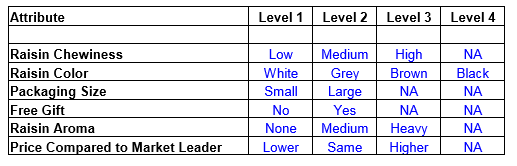
\includegraphics[width=8cm]{q1.PNG}
%\end{center}



\begin{itemize}
\item \textbf{[1c] What is the probability of awareness for someone who watches 20 hours of TV, made 8 detergent purchases last year, is female, and makes \$60,000? }
\end{itemize}

$$  \mathlarger{ \hat{Y} = \hat{p}_{AwareCSG} = \hat{p}(x_1,x_2,x_3,x_4) = \frac{e^{\hat{\beta}_0 + \hat{\beta}_1 x_1 + \hat{\beta}_2 x_2 + \hat{\beta}_3 x_3 + \hat{\beta}_4 x_4 }}{1 + e^{\hat{\beta}_0 + \hat{\beta}_1 x_1 + \hat{\beta}_2 x_2 + \hat{\beta}_3 x_3 + \hat{\beta}_4 x_4 }}}$$
% Juan: we can probably expect that all variables will be selected - simply fill in the values for these coefficient values

$$  \mathlarger{ \Rightarrow \hat{p}_{AwareCSG} = \hat{p}(20,8,0,\$60k) = 0.006447225 \approx 0.64\% }$$

See Appendix 4.2 for R code.

\pagebreak

\begin{itemize}
\item \textbf{[1d] How does the probability of awareness change with more hrs of TV watching? Plot the probability of awareness as the amount of TV watching varies from 0-50 hrs per week. You can plot the probability of awareness using increments of 5 hrs (for the analysis, assume 8 detergent purchases last year, female, and income of \$60,000).  } 
\end{itemize}


\begin{center}
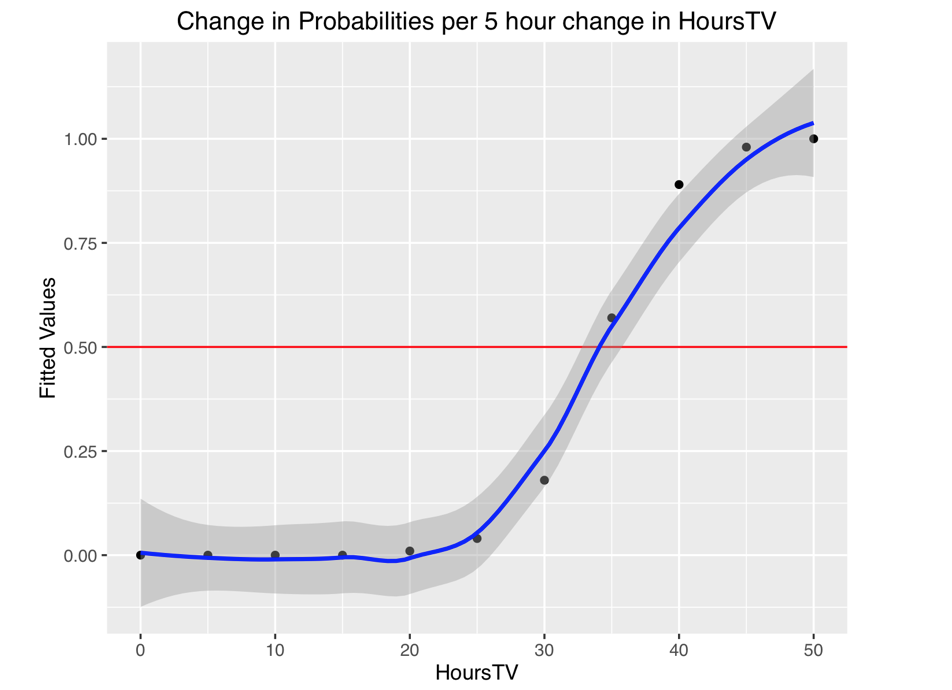
\includegraphics[width=15cm]{1d.png}
\end{center}



From the model coefficients, we know that a unit increase in \textbf{'Hours TV'} results in an increase of $ \approx 0.35$ in log-odds. As we can see in the plot above, there is a steep increase in $\hat{p}(20,8,\Delta x_3,\$60k)$ for $x_3 > 25 $, with $\hat{p} \geq 0.5 $ when $x_3 \geq  34 $ (See Appendix 4.3 for R code)
%\begin{center}
%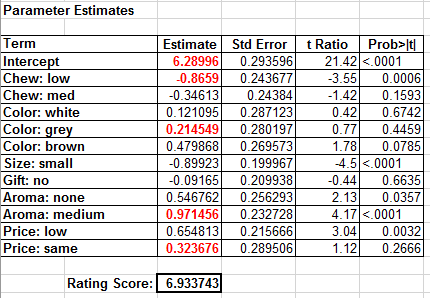
\includegraphics[width=8cm]{1d.PNG}
%\end{center}

\pagebreak


\begin{itemize}
\item \textbf{[1e] Do the independent variables as a whole, in your model, provide statistically significant explanatory power at 5\% level for predicting the probability that someone is aware of CSG?  State how you arrived at this conclusion based on your regression output.}
\end{itemize}

$$ H_0 : \textrm{Logistic Regression Model with all variables adequately fits the data  }$$
$$ H_a : \textrm{Logistic Regression Model with all variables does not provide an adequate fit } $$

To measure goodness of fit, a Hosmer–Lemeshow (H.L.) test is a good method for this particular. An H.L. test is a statistical test for goodness of fit for logistic regression models, developed by Hosmer and Lemeshow (1980), frequently used in risk prediction models. It assesses whether or not the observed event rates match expected event rates in subgroups of the model population. $H_0 $ can be redefined in this situation as \textit{"actual and predicted event rates are similar across 10 deciles"}. If $p_{H.L.} > \alpha; \alpha = 0.05 $, we reject $H_0$.

\begin{center}
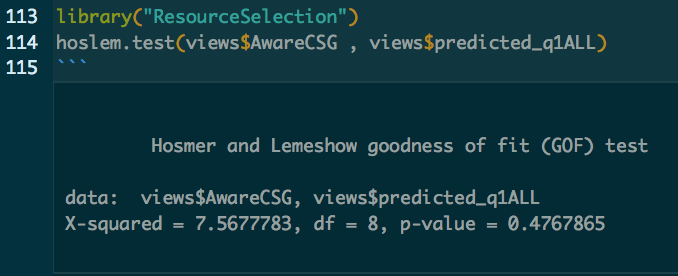
\includegraphics[width=12cm]{hltest.png}
\end{center}

The test finds that our full model, as indicated by $p_{H.L.} \approx 0.477 >> 0.05 $, \textit{\textbf{does not properly fit the data}}. In consequence, we should rethink our model, and include interactions to see if the fit improves.


\pagebreak


\begin{itemize}
\item \textbf{[1f] State two ways that CSG can use the results of this regression equation in a managerial way.  Be as specific as you can be.}
\end{itemize}

\begin{table}[ht]
\caption{ Results - Full Model} % title of Table
\centering % used for centering table
\begin{tabular}{l c c c c} % centered columns (4 columns)
\hline\hline %inserts double horizontal lines
Predictor Variable & $\beta_j $ & \textbf{$Pr(>\mid z \mid )$} & Significant at $\alpha = 0.02$ & Significant at $\alpha = 0.01$ \\ [1.5ex] % inserts table
%heading
\hline % inserts single horizontal line
$x_1:$ Hours TV  &  $\approx 0.3531  $ & $ \approx 2.04 \cdot 10^{-21}$ & Yes & Yes \\ % inserting body of the table
$x_2: $ DeterPur  &  $\approx -0.9967  $ & $ \approx 1.00 \cdot 10^{-16}$ & Yes & Yes  \\
$x_3:$  Gender &  $\approx -0.4792  $ & $ \approx 2.33 \cdot 10^{-2}$& No & No  \\
$x_4:$  Income  &  $\approx -4.12 \cdot 10^{-4} $& $ \approx 6.65 \cdot 10^{-9}$ & Yes & Yes    \\[1ex] % [1ex] adds vertical space
\hline %inserts single line
\end{tabular}
\label{table:full} % is used to refer this table in the text
\end{table}

%#                  Estimate   Std. Error   z value     Pr(>|z|)

%#HoursTV       0.3531541866 3.716322e-02  9.502787 2.043471e-21
%#DetergentPur -0.9967498367 1.200227e-01 -8.304675 1.000932e-16
%#Gender       -0.4791504419 2.112639e-01 -2.268018 2.332809e-02
%#Income       -0.0004121295 7.106113e-05 -5.799648 6.645422e-09

The results of our full model are described in Table 2 above. The sorted coefficients in terms of their absolute values are $\beta_2  > \beta_3 > \beta_1 > \beta_4 $. While $X_2$ is not significant at $ \alpha = 0.02$, it is fairly close. See Appendix 4.4 for R code. This information overall can be used in several ways, such as:

\begin{enumerate}
\item As seen in 1(d) and as reflected by $\beta_1$, on average, people who watch more TV (controlling for other factors) are much more likely to be aware of the new detergent brand. \textit{\textbf{Thus, based on this information, marketing campaigns should target demographics with high exposure to media through television (reflected by a high $X_1$).  }}
\item As reflected by $\beta_3$, controlling all factors but gender,  men are less likely to be aware of new detergent brands. \textit{\textbf{Thus, based on this information, marketing campaigns should target women either exclusively or to a much larger extent than men. }}
\end{enumerate}


\pagebreak

\begin{itemize}
\item \textbf{[1g] Managers also care about how two variables may interact with other each. Include an interaction between the two variables “Gender” and “TV watching” in the above model and estimate the regression coefficients. Describe your results. Using the coefficients, calculate the following:}
\end{itemize}
%0.006994688203*100 = 0.6994688203
%0.003592422942*100 = 0.3592422942

\begin{table}[ht]
\caption{ Results - Full Model with interactions between 'HoursTV' and 'Gender'*} % title of Table
\centering % used for centering table
\begin{tabular}{l c c c c} % centered columns (4 columns)
\hline\hline %inserts double horizontal lines
Predictor Variable & $\beta_j $ & \textbf{$Pr(>\mid z \mid )$} & Significant at $\alpha = 0.02$ & Significant at $\alpha = 0.01$ \\ [1.5ex] % inserts table
%heading
\hline % inserts single horizontal line
$x_1:$ Hours TV &  $\approx 0.3114  $ & $\approx 3.25\cdot 10^{-15}$ & Yes & Yes \\ % inserting body of the table
$x_2: $ DeterPur & $\approx -0.9908  $ & $\approx 2.8\cdot 10^{-16}$ & Yes & Yes \\
$x_3:$  Gender & $\approx -2.530  $ & $\approx 1.08\cdot 10^{-3}$ & Yes & Yes \\
$x_4:$  Income & $\approx 4.16\cdot 10^{-4}$ & $\approx 1.01\cdot 10^{-8}$ & Yes & Yes   \\% [1ex] adds vertical space
$x_5*:$  $x_1 \leftrightarrow x_3$ & $\approx 0.093  $ & $\approx 0.0056$ & Yes & Yes  \\[1ex]
\hline %inserts single line
\end{tabular}
\label{table:allpredint} % is used to refer this table in the text
\end{table}

%                      Estimate       Std. Error      z value                    Pr(>|z|)
%(Intercept)    -3.231890532898 0.55873061021974 -5.784344859 0.0000000072795468903305581
%HoursTV         0.311369072746 0.03950920798393  7.880924185 0.0000000000000032496844740
%DetergentPur   -0.990767510674 0.12109629359348 -8.181650167 0.0000000000000002799828999
%Gender         -2.530082223654 0.77405994389859 -3.268586940 0.0010808596544437071122757
%Income         -0.000415596951 0.00007253816788 -5.729355499 0.0000000100812923840726538
%HoursTV:Gender  0.093016885269 0.03354975924882  2.772505298 0.0055626613883063341300939

The results of our full model with interactions are described in Table 3 above. The sorted coefficients in terms of their absolute values are $\beta_3  > \beta_2 > \beta_1 > \beta_5 > \beta_4 $. After including the interaction between $X_1$ and $X_3$, this model adds more weight to the effect of gender on the log-odds of $\hat{Y} = \hat{p}_{AwareCSG}$. Running another H.L. test gives us $p_{H.L.} \approx 0.1494$, showing that fit has improved compared to the previous model, but is still not sufficient (a model with all interactions, $x_1 \leftrightarrow x_2,x_3,x_4 $ outputs $p_{H.L.} < 0.05$  ). Nevertheless, for the purpose of this exercise, this model will suffice. See Appendix 4.4 for the corresponding R code.


\begin{enumerate}
\item \textbf{What is the probability of awareness for someone who watches 20 hours of TV, made 8 detergent purchases last year, is female, and makes \$60,000? }

$$  \mathlarger{ \Rightarrow \hat{p}_{AwareCSG} = \hat{p}(20,8,0,\$60k) = 0.006994688203 \approx 0.70\% }$$


\item \textbf{What is the probability of awareness for someone who watches 20 hours of TV, made 8 detergent purchases last year, is male and makes \$60,000? }
\end{enumerate}

$$  \mathlarger{ \Rightarrow \hat{p}_{AwareCSG} = \hat{p}(20,8,1,\$60k) = 0.003592422942 \approx  0.36\% }$$

As we can see in this particular example, our model predicts that the probability of awareness for a woman who watches 20 hours of TV, made 8 detergent purchases last year, is female, and makes \$60,000 is almost twice that of a man with the same characteristics. 

\pagebreak

\section{Survey Analysis}

\textit{We will revisit a dataset that we used in the previous assignment – the survey of a sample of supermarket owners for their opinions on the raisin industry, and conduct a deeper analysis.}

\begin{itemize}
\item \textbf{[2a] Run a 3-means clustering on $ Q_{1},...,Q_{9} $. What appear to be the significant drivers of variation between the groups? How would you statistically test what the significant drivers are between groups?   }
\end{itemize}

\begin{center}
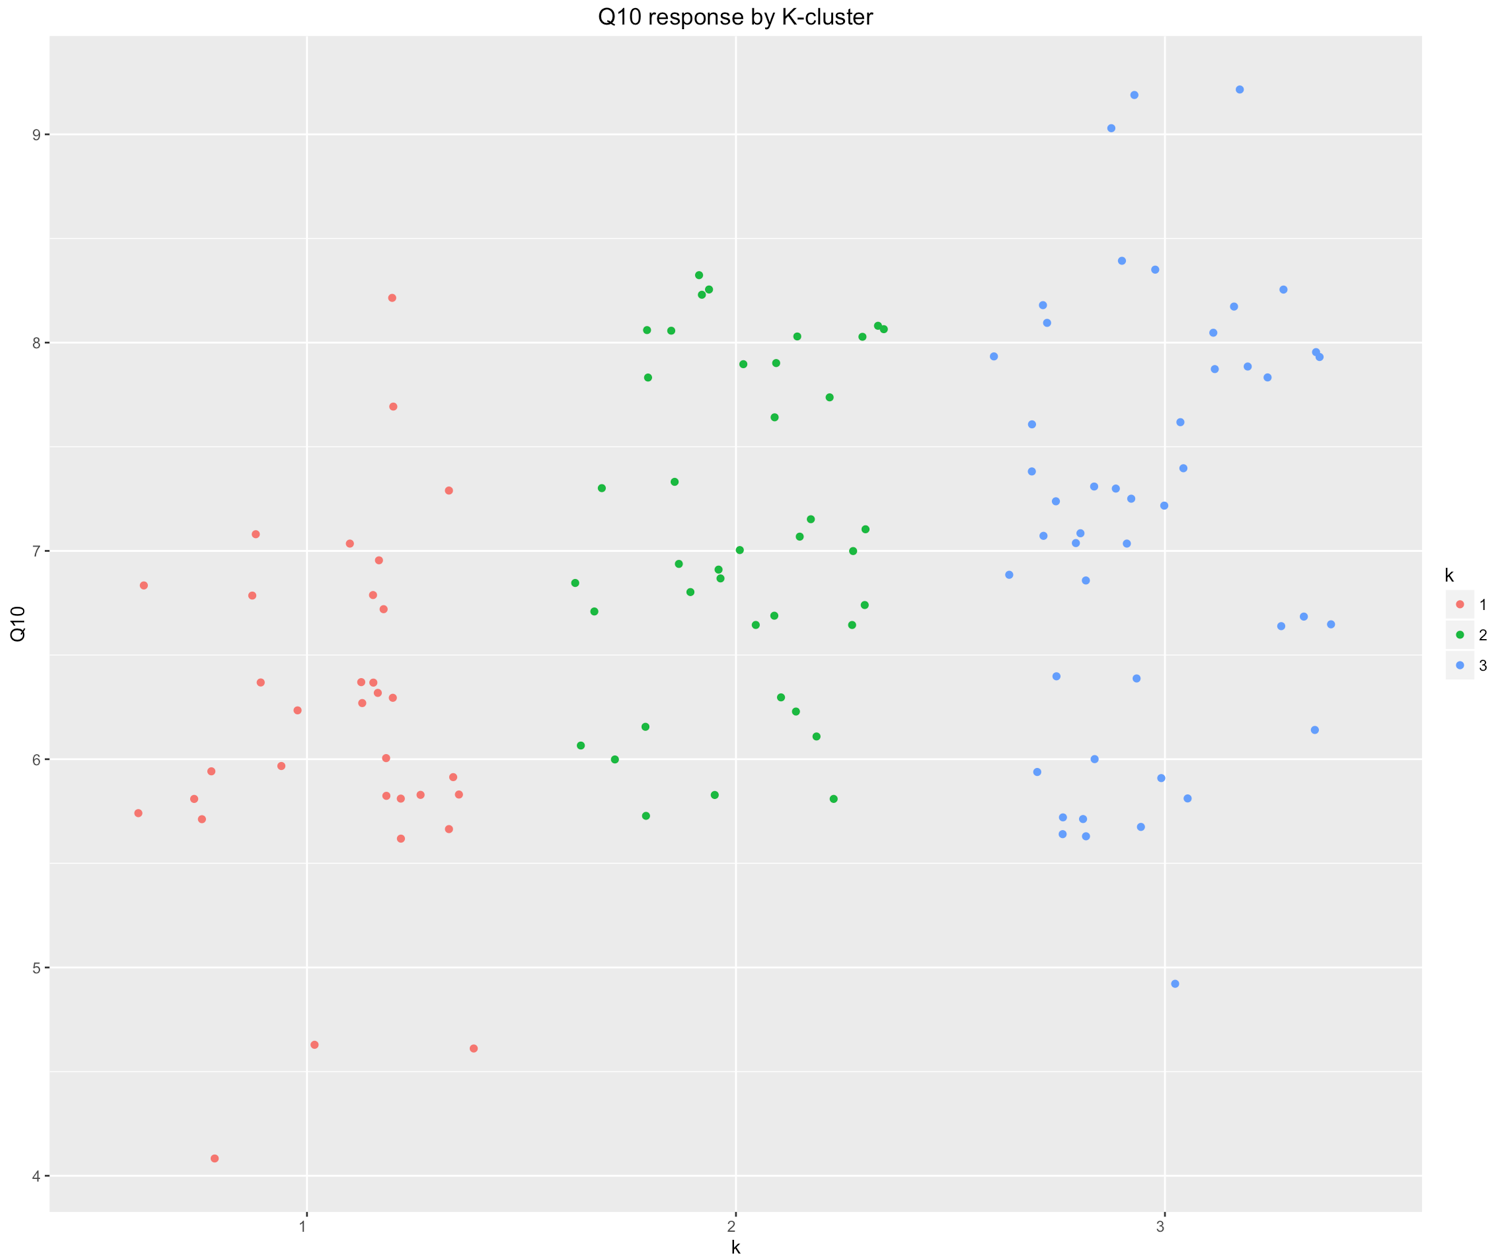
\includegraphics[width=12cm]{clusters.png}
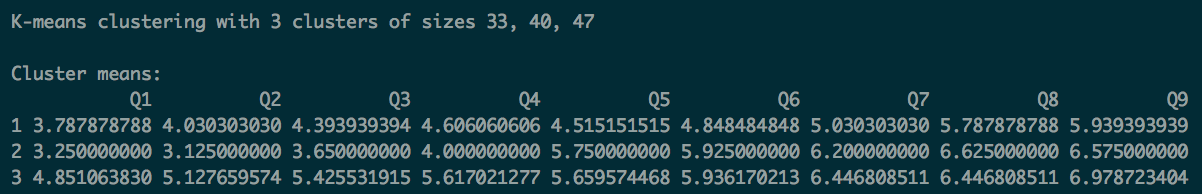
\includegraphics[width=15cm]{knn.png}
\end{center}

We ran a 3-means clustering on $X: Q_{1},...,Q_{9} $ (See Appendix 4.6). The results and a plot of $Y: Q_{10}$ per each $k$-cluster show differences in $X,Y$. At a glance, some question's mean response per cluster do not seem to follow the same ordinal ranking as the response. $Q_{4}$, \textit{"Giving away in-package free gifts is a strong driver of brand sales."}, for instance, is predictive when regressing the joint sample, but this could change once we run a regression on each cluster - comparing the $t$-values would allow us to statistically test what the significant drivers are between clusters.

\begin{itemize}
\item \textbf{[2b]   For each of the 3 segments, which variables (out of $ Q_{1},...,Q_{9} $) are significant predictors, at the 10\% significance level, of Q10, the overall profitability in the raisin category?  Clearly, describe how the 3 segments are different in terms of what matters for profitability. Also, compare the above results with those from the entire dataset. What are the big differences?   }
\end{itemize}
\begin{center}
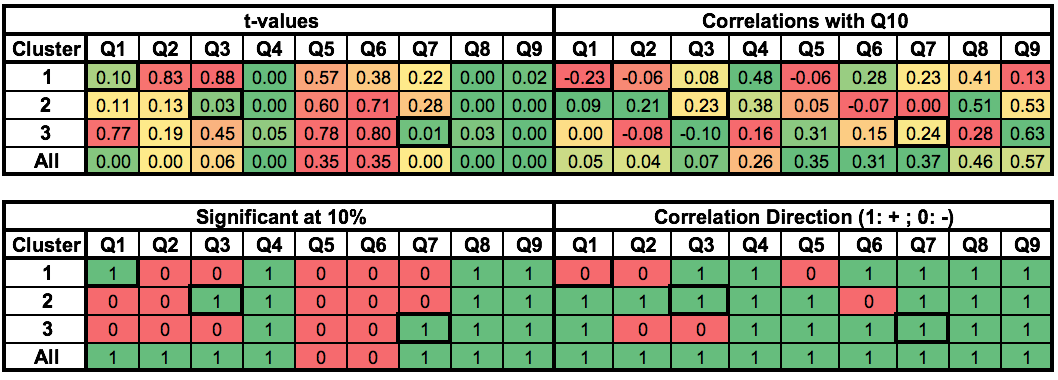
\includegraphics[width=15cm]{2b1.png}
\end{center}
We ran separate OLS regressions for $X: Q_{1},...,Q_{9} $, for each of the $k = 1,2,3 $ clusters and for the joint data. The results are summarized on the tables above. The first table shows the $t$-values and correlations with $Q_10$ for each cluster and for all clusters. The second table indicates whether or not $Q_j$ is statistically significant for a given $k$ or all $k$'s, with $X_{k,Q_{j}} = [1: \alpha > Pr(>\mid t_{k,Q_{j}} \mid ) ]; 0: \alpha < Pr(>\mid t_{k,Q_{j}} \mid )  $ for $\alpha = 0.1 $, and whether the correlation is positive or negative. We make the following observations:
\begin{enumerate}
\item $Q_{4}$,$Q_{8}$ and $Q_{9}$ are significant at $\alpha = 0.1$ for any $k$ as well as for the joint data, and $Q_{5}$ and $Q_{6}$ are not significant at $\alpha = 0.1$ for the same groups.
\item While $Q_{2}$ is statistically significant at $\alpha = 0.1$ for the joint data, it is not significant in any of the $k$-cluster regressions.
\item \textbf{ Thus, the likely drivers of variation between the $k$-clusters are $Q_{1}$ for $k=1$, $Q_{3}$ for $k=2$, and $Q_{7}$ for $k=3$, as indicated in the second table with the cells outlined in bold. }
\end{enumerate} 

Now that we have identified our likely drivers, we need to interpret the implications for each cluster based on the available information. We can make some inferences regarding the differences between clusters in Supermarket Owner's strategies, based on the $t$-values, coefficients and correlations from our different regression models:
\begin{enumerate}
\item For owners in $k=1$, the more value the raisins' color, on average, the lower their $Q_{10}$ response. This is evidenced by the $t$-value, the negative correlation, and  $\beta_{k=1,Q_{1}} \approx -0.3 < 0$. We could interpret this as a sign of these owner's over-emphasizing details of their merchandise that have a small effect on their sales, explaining the disconnect with profitability.
\item On average, owners in $k=2$ that signal caring about offering a variety of package sizes, or allow customers to purchase custom quantities, charging per pound (or kilo) sold, for example, will tend to have a higher $Q_{10}$ response. This is evidenced by the $t$-value, the positive correlation, and the coefficient, $\beta_{k=2,Q_{3}} \approx 0.284$. 
\item  On average, owners in $k=3$ that see raisins as sales catalysts (complementary to the sales of other fruits), will tend to have a higher $Q_{10}$ response. This is evidenced by the $t$-value, the positive correlation, and the coefficient, $\beta_{k=3,Q_{7}} \approx 0.24$. 
\end{enumerate}
 
 There are several caveats to this analysis - small sample size and non-standardized values, for instance, do not allow us to compare coefficients directly. But there is clear value to be gained on using these statistical methods on larger samples. 


\begin{itemize}
\item \textbf{[2c] Based on the above comparison, please explain (as simply as possible) why regression analysis and segmentation together can provide a lot more insight into underlying drivers as opposed to a single regression model for the entire market place. }
\end{itemize}

%\begin{center}
%\includegraphics[width=15cm]{q137.png}
%\end{center}

As we see in the results and the analysis on 2(a) and 2(b), there are non-negligible differences between the joint analysis of Storeowner's responses and the cluster-level analyses. Performing regression analysis and segmentation together introduces a higher level of heterogeneity to the exercise, allowing for deeper insights and consequently, more precise marketing. It also helps avoid reaching the wrong conclusions (and acting on them). 
 
 







\pagebreak

\section{Customer Engagement Data}

\textit{ We are very interested in understanding what the variables are for predicting whether a customer will engage with an ad or email (“Engagement”). Please answer the following questions.}

\begin{itemize}
\item \textbf{[3a] How does the timing of the impression (when it is sent) impact the probability that a customer will engage? How does the probability of engagement vary by month, time of day, day of the week? In other words, please document the temporal variation of engagement. This analysis can help managers decide when to send an impression.   }
\end{itemize}

We split the data set by month to compare and contrast, and ran logistic regressions predicting $Y: \textrm{Engagement}$ with $X_{(i)}: \textrm{Hour of Day} $ and $X_{(ii)}: \textrm{Day of the Week} $. We then ran a logistic regression with $X_{(iii)}: \textrm{By Month} $ using the joint data. 

\textbf{\textit{(i) Engagement by Hour of Day:}}
\begin{center}
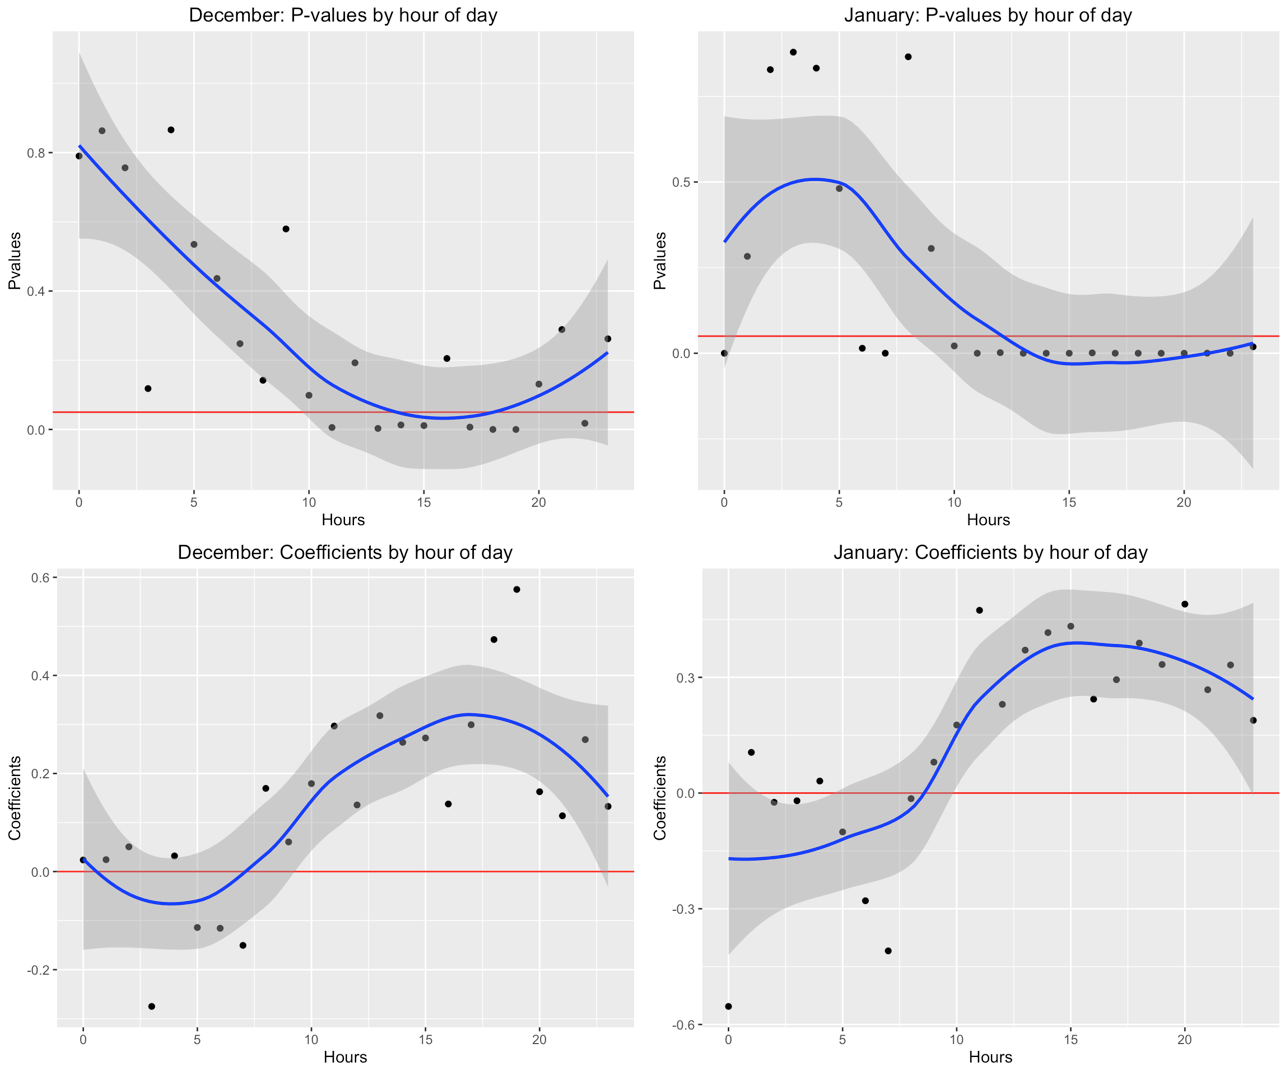
\includegraphics[width=14cm]{hod.png}
\end{center}

\textbf{\textit{(ii) Engagement by Day of the Week:}}
\begin{center}
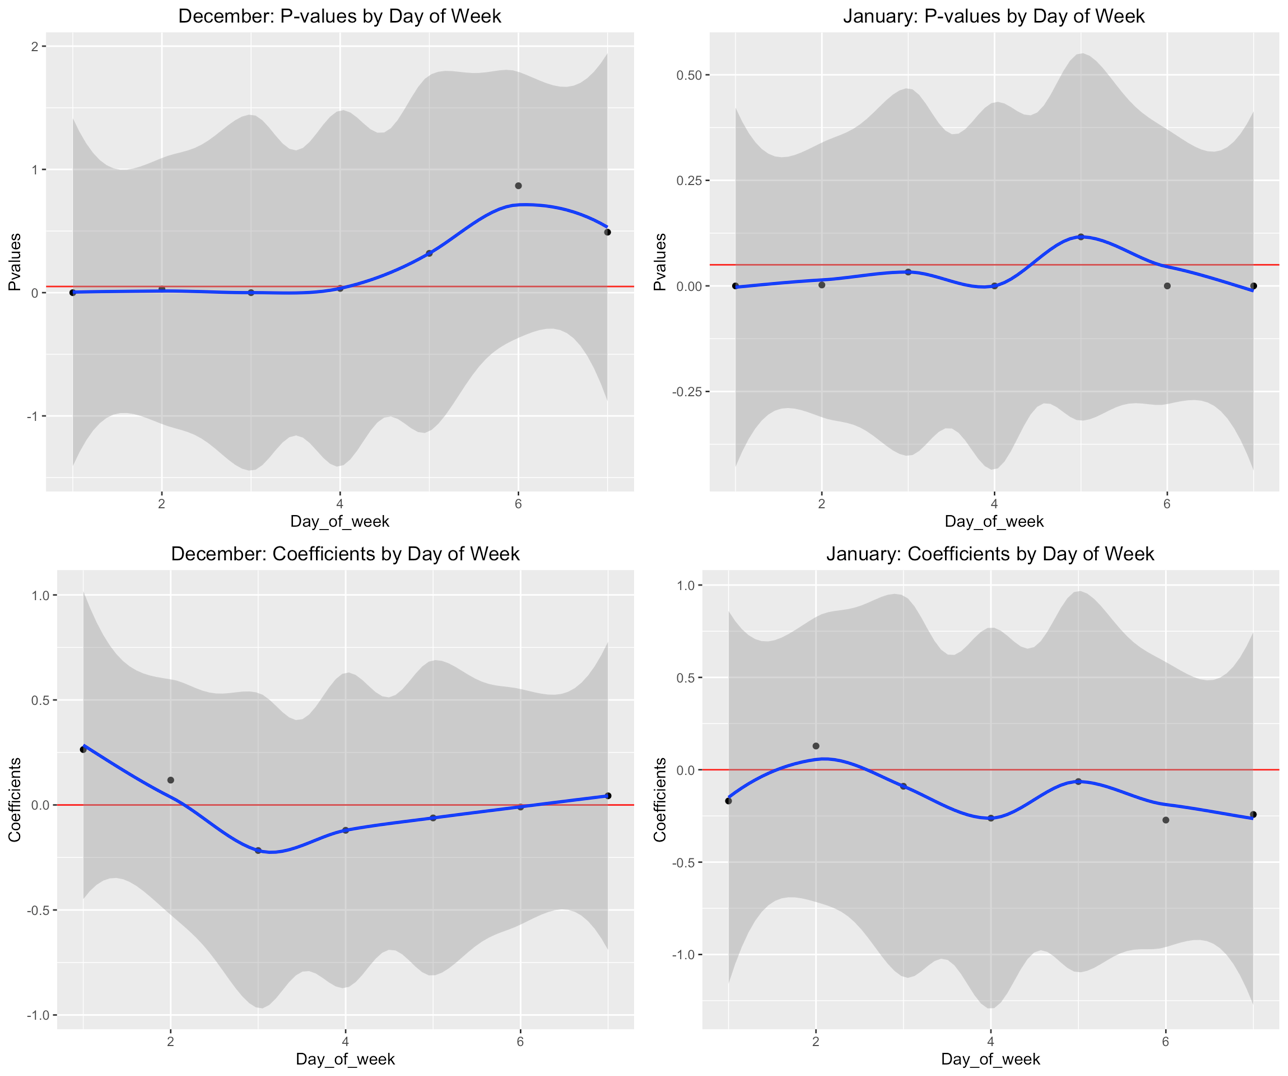
\includegraphics[width=13cm]{dow.png}
\end{center}

\textbf{\textit{(iii) Engagement by Day of the month:}}
\begin{center}
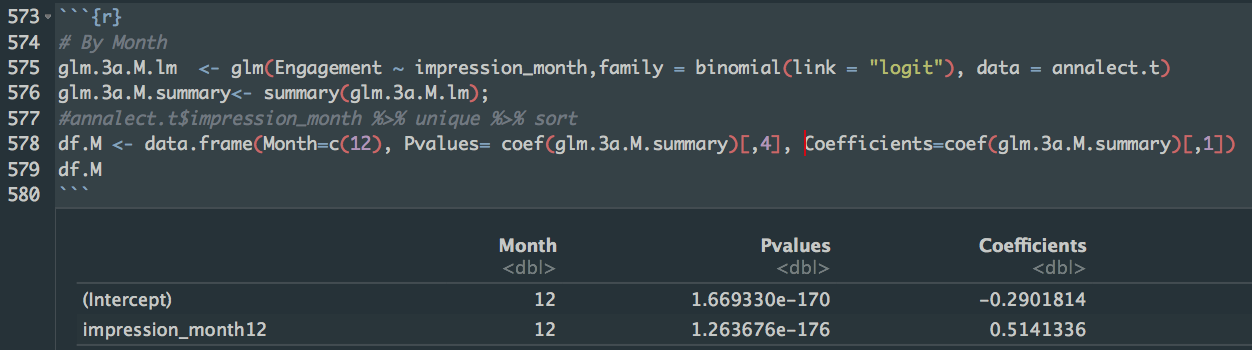
\includegraphics[width=13.5cm]{month.png}
\end{center}


Through the scatter plots showing how engagement varied at different times of day, for both January and December separately, we can identify the key times of day to increase probability of engagement. It seems as though engagement is generally more variable and higher at peak hours in January than in December.  For both months, late afternoon (6:00 pm - 8:00 pm) was the time of highest engagement, and engagement increased markedly after around 10:00 am on both months.  The lowest engagement was found at midnight in January, and around 4:00 am in December.  In both December and January the trend is a general increase in engagement as the 24-hour day progresses, but there's a dip in engagement  in the early hours of the morning (before about 7:00 am).

It's also useful to look at how engagement varied by day of the month.  For both December and January, engagement was highest at the beginning of the month and declined all the way to the end (with a slight bump up in the last five or so days of the month).  However, the first five days of January have a steep decline that is only seen from the first day to the second day of December.  

Finally, we examine variation by day of the week.  In December, engagement rapidly decreases from Sunday to Monday and Monday to Tuesday, reaching its low on Tuesday.  For there there is a steady increase in engagement until the end of the week.  Engagement by weekday is more variable in January - engagement is at its highest on Monday and decreases to a Wednesday low before spiking back up to near Tuesday levels on Thursday, reaching a low again on Friday, and increasing slightly through Sunday.  From this data we can draw the conclusion that the best time to send an impression would be around 7:00 pm on a Sunday at the beginning of December or on a Monday at the beginning of January.   


\begin{itemize}
\item \textbf{[3b]   We also want to understand the impact of creatives on engagement. Since there are many creatives (which you can check if you assess the distribution), it will be difficult to carry out an analysis for every creative. Thus, I would like you to focus on the creatives that were sent to more than 5\% of people (each line in the dataset is a person). Consider all creatives that are sent to less than 5\% of people as “the baseline level”. Of the creatives that were sent to more than 5\% of people, I would like you to quantify how the creative impacts the probability of their engagement (whether they engage or not).    }
\end{itemize}


\begin{enumerate}
\item \textbf{Are some creatives better than others for engaging customers? If so, which ones? }
\item \textbf{Are email-based creatives better than other types of creatives? Please summarize your findings about the importance of different types of creatives as best as you can.  }
\end{enumerate}

\textbf{Please note that this last question is a bit open ended and not as structured (capturing the spirit of what clients typically ask from companies doing analytics). I am interested in seeing how you approach the problem.} 

\textbf{\textit{3b(1) Impact of creatives on Engagement}}
\begin{center}
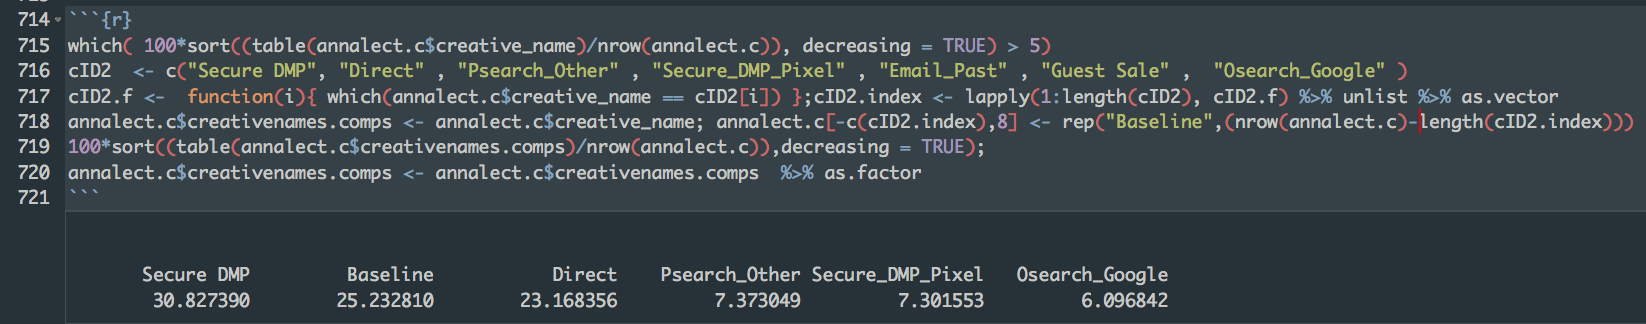
\includegraphics[width=14cm]{3bi1.png}
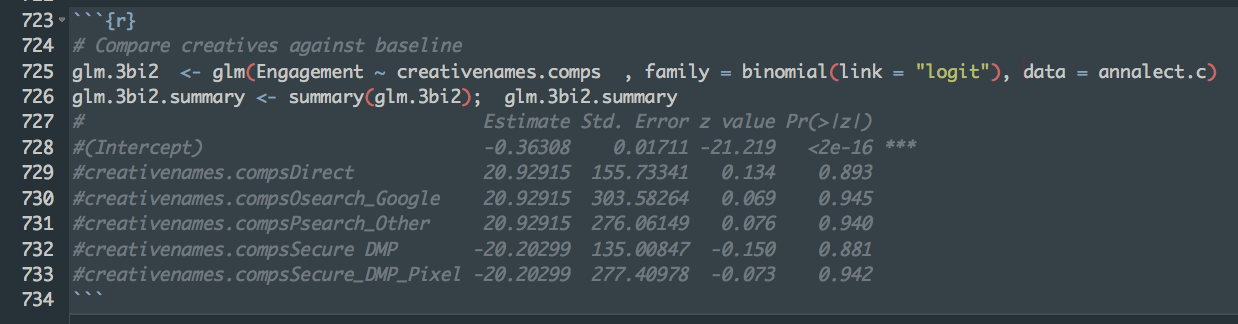
\includegraphics[width=14cm]{3bi2.png}
\end{center}
We created a custom variable, $'creativenames.comps'$, where all $'creative\_names'$ aggregating less than 5\% of engagements are encoded as "\textit{Baseline}". None of the non-baseline creatives have significant $p$-values, but $\beta_{0,3b(1)}$ is quite significant. This was quite odd at first, and we will explain why we think this is the case after our results for \textbf{3b(2)}.
\medskip

\textbf{\textit{3b(2) Impact of email-based creatives on Engagement}}
\begin{center}
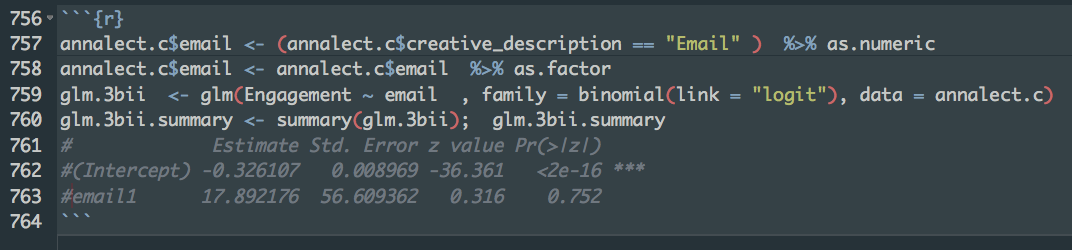
\includegraphics[width=14cm]{3bii1.png}
\end{center}
We created a custom variable, $'email'$, where all email-based creatives are encoded as \textbf{"1"} and the remaining 44 types are encoded as \textbf{"0"}. Just as in \textbf{3b(1)}, none of the email-based creatives have significant $p$-values, but $\beta_{0,3b(2)}$ is significant. We believe this is due to a problem with the data, as we will explain in the next page.

\pagebreak
\textbf{\textit{3b Discussion: possibility of an unrepresentative sample}}
\begin{center}
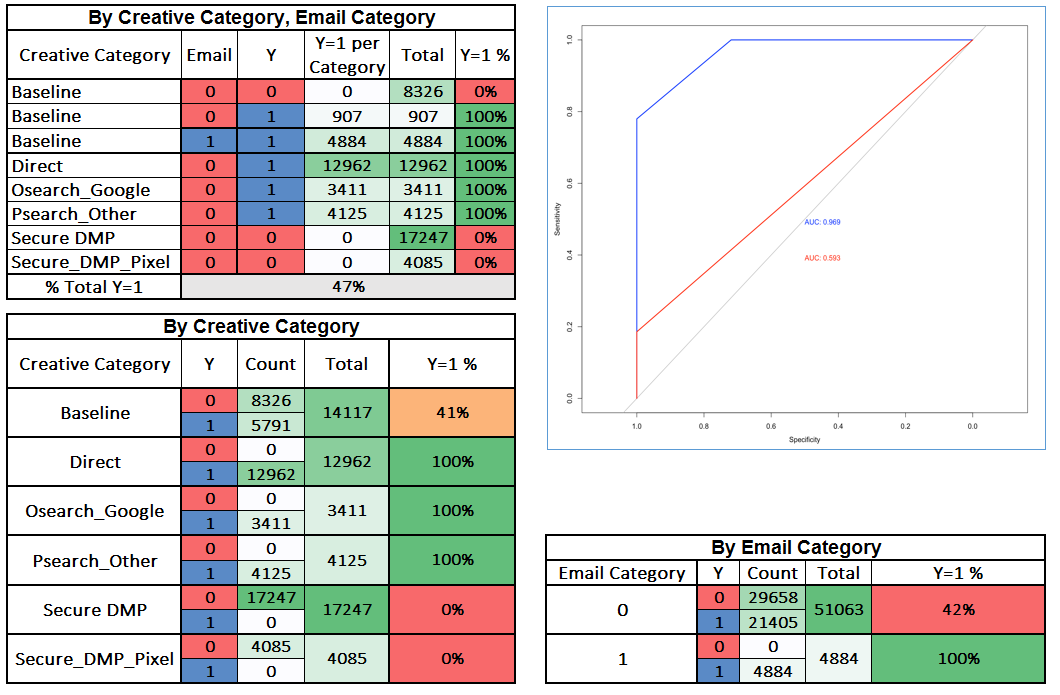
\includegraphics[width=12cm]{3results.png}
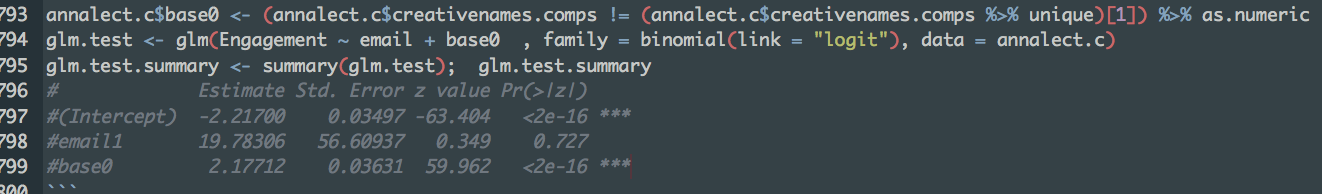
\includegraphics[width=14cm]{base0.png}
\end{center}

By aggregating the results via R's $'dplyr'$ package, we are able to get a sense of what the problem could be. The first red flag is the proportion of engagements, $\frac{\sum_{i=1}^{55947} Y_i = 1}{55947} \approx 47\%$. It seems unrealistic to expect almost half of the exposures in a representative sample to lead to engagements, so either the dataset does not contain random users, or contains too few observations to be representative. It is extremely unlikely that non-baseline creative have either 0\% or 100\% success rates in a representative sample. The same applies to email-based creatives having a 100\% success rate in a representative sample. We note that only baseline creatives with $<5\%$ of activity sent email advertisements. Running a final logistic regression on comparing baseline versus non-baseline as well as email and non-email as binary predictor variables, tells us is that email has a higher success rate for baseline creatives, as we can see by the regression results. The fitted values for baseline creatives, $\hat{p}_{B}$ are $\hat{p}_{B,E} \approx  99.9\% $ and $ \hat{p}_{B,NE}  \approx 9.8\%$ for email and non-email based types, respectively, and $ \hat{p}_{NB} \approx 49\% $ for non-baseline creatives (none of which sent email-ads). So while it seems that email works better as a channel for $\approx 25.2\% $ of the sample (baseline creatives), our doubts regarding the quality of the data do not allow us to conclude whether or not non-baseline creatives necessarily outperform baseline ones. 



\pagebreak
\section{Appendix}



\subsection{R Outputs for Q1(a,b)}

\begin{center}
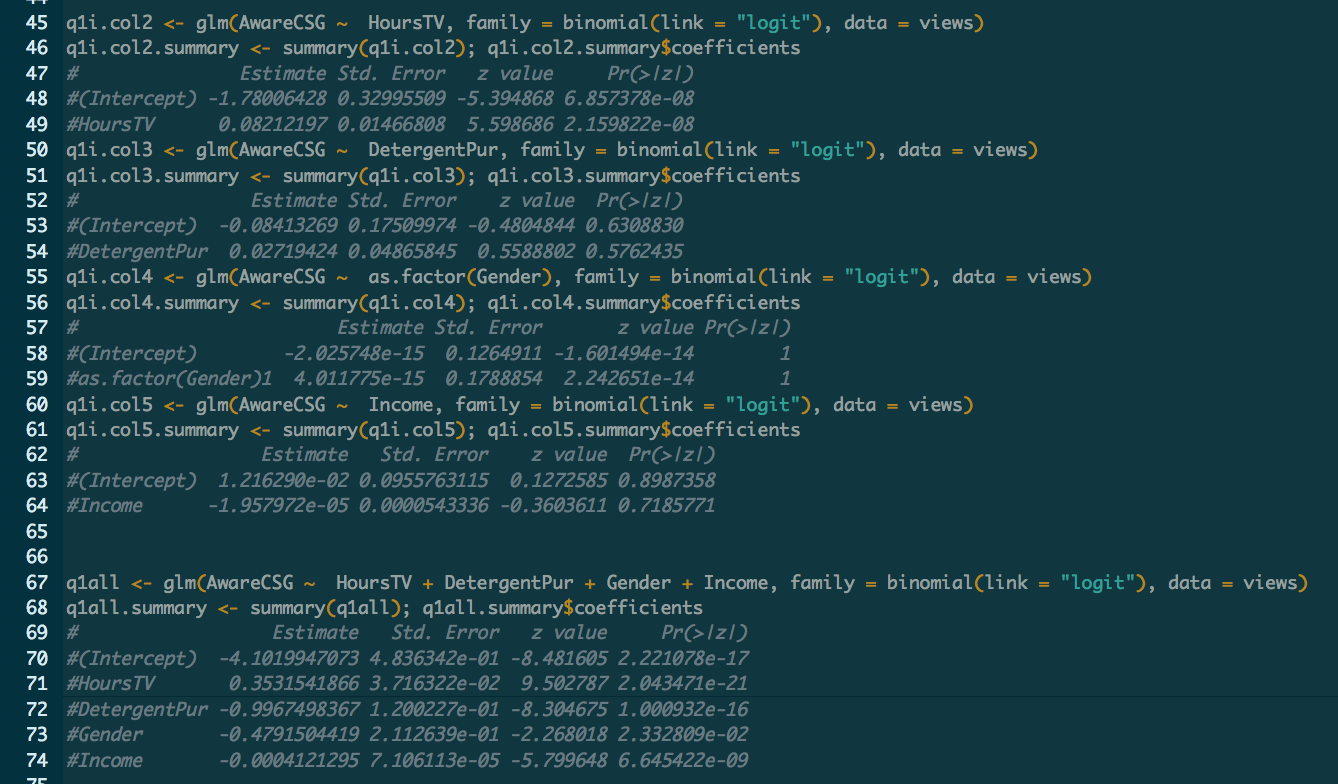
\includegraphics[width=16cm]{1a.png}
\end{center}

\subsection{R Outputs for Q1(c)}

\begin{center}
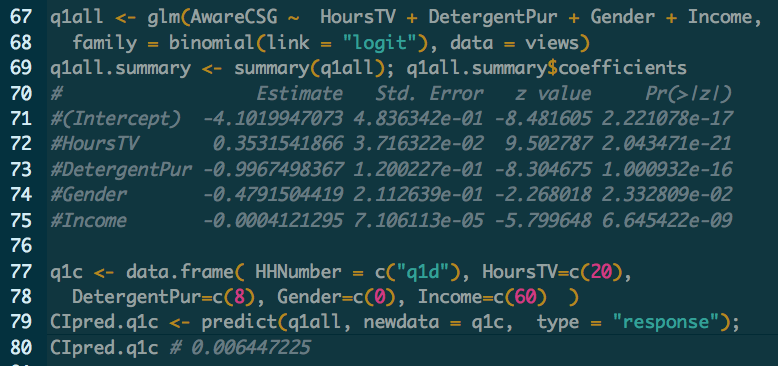
\includegraphics[width=14cm]{1all.png}
\end{center}


%\begin{center}
%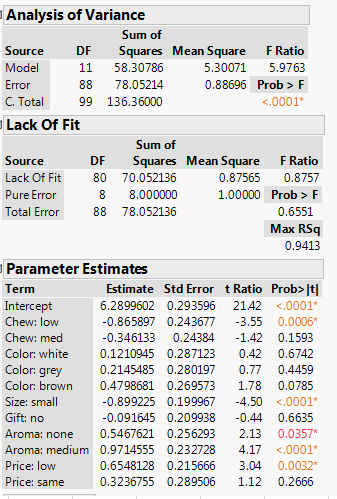
\includegraphics[width=8cm]{1j.PNG}
%\end{center}

\pagebreak

\subsection{R Outputs for Q1(d)}

\begin{center}
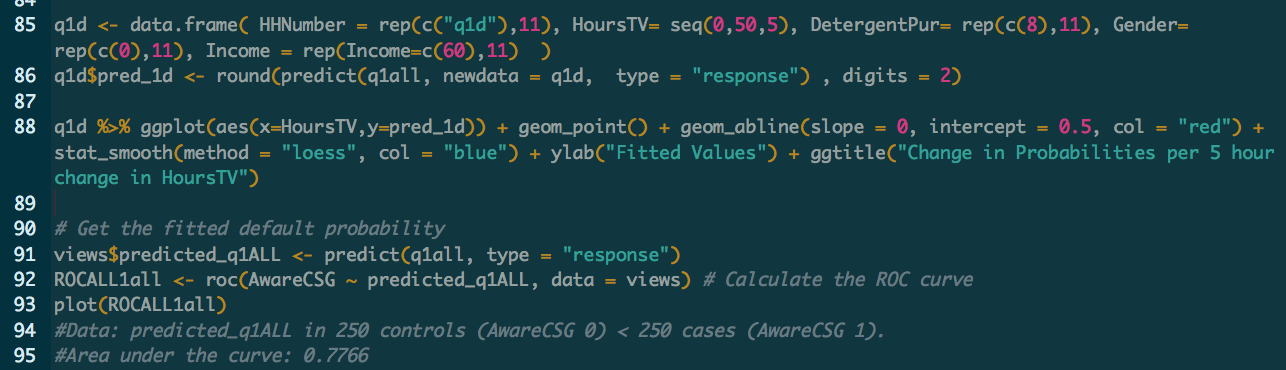
\includegraphics[width=15cm]{1dcode.png}
\end{center}

%\begin{center}
%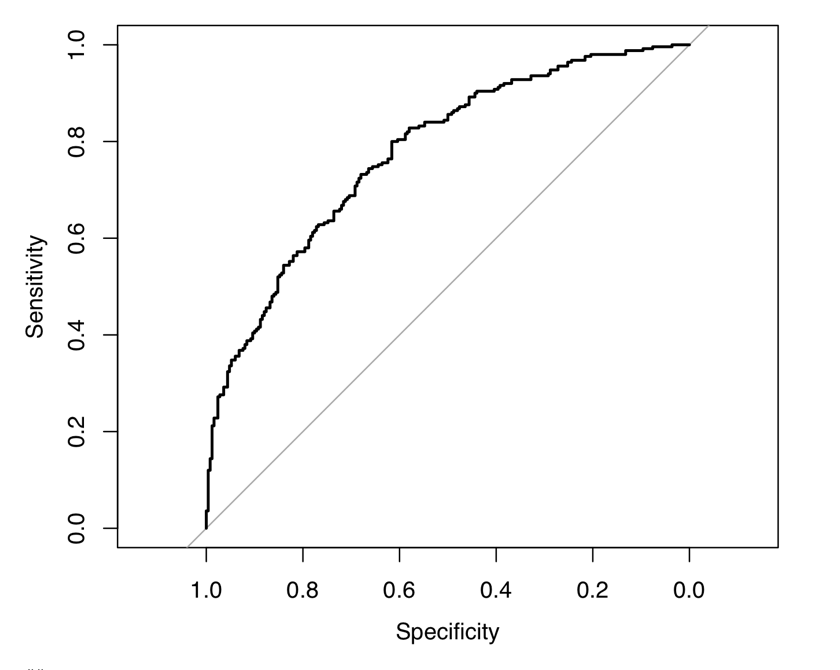
\includegraphics[width=12cm]{ROC1.png}
%\end{center}

\subsection{R Outputs for Q1(f,g)}


\begin{center}
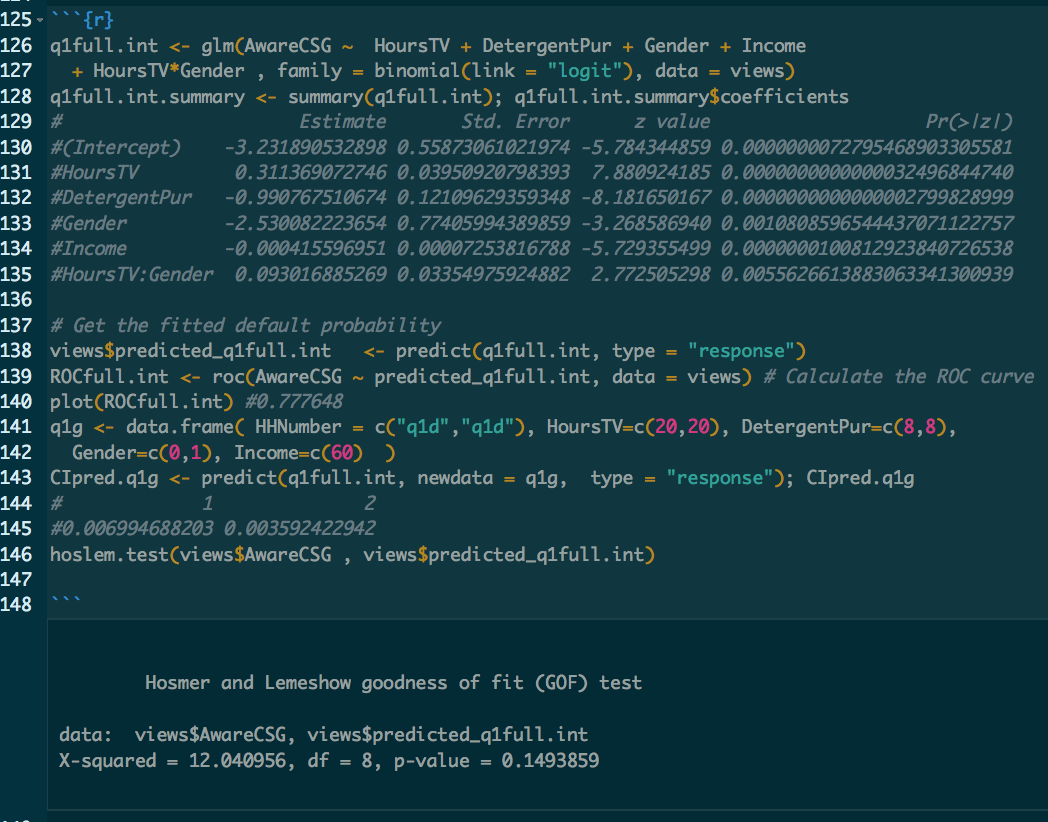
\includegraphics[width=16cm]{intmodel.png}
\end{center}

%\begin{center}
%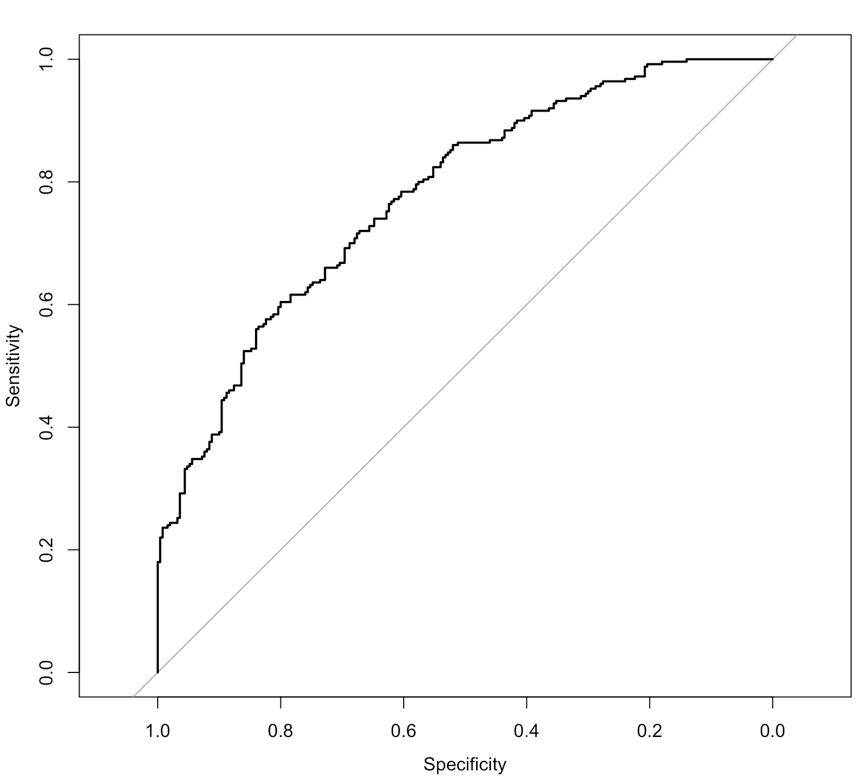
\includegraphics[width=10cm]{ROC2.png}
%\end{center}



\pagebreak

\subsection{Supermarket Owner Questionnaire}


Please answer each of the following questions on a 1-10 scale where 1 indicates that you disagree completely with the given statement and 10 indicates perfect agreement.
\begin{enumerate}


\item Raisin color is a key determinant of raisin category sales.
\item Raisin aroma is a key determinant of raisin category sales.
\item Raisin consumers have differing preferences for varying raisin package sizes.
\item Giving away in-package free gifts is a strong driver of brand sales.
\item Raisin consumers are price sensitive.
\item Raisin chewiness is an important determinant of raisin preference.
\item Raisin sales are highly linked to the sales of other fruits.
\item Marketing for the raisin category can significantly affect people’s purchasing habits.
\item I enjoy raisins as part of my daily diet.
\item The raisin category is extremely profitable in my store.

\end{enumerate}

Additional Questions: 

What is the monthly dollar volume of your store?
How much marketing expenditure, per month, do you spend on the raisin category?
How many different SKUs of raisins does your store carry?

\pagebreak

\subsection{Q2(a,b) R Code }

\begin{center}
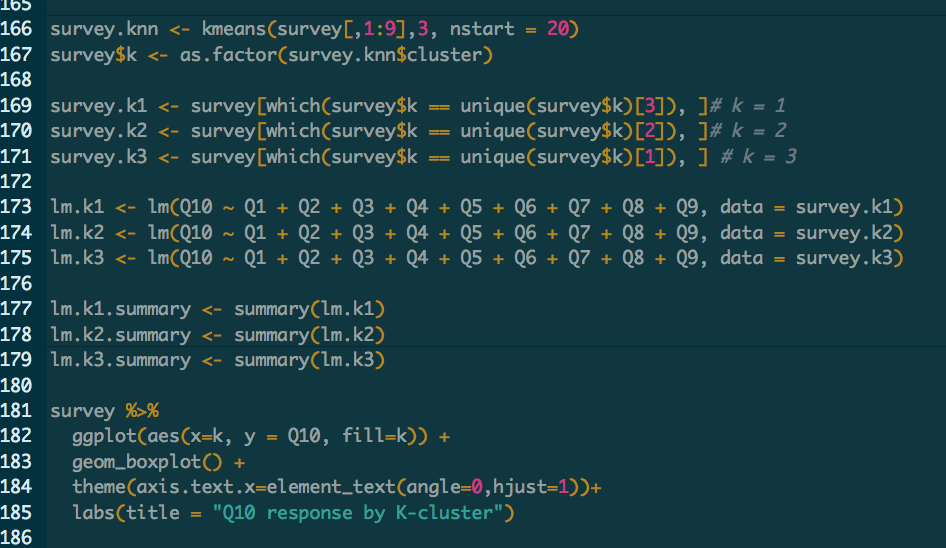
\includegraphics[width=16cm]{2a1.png}
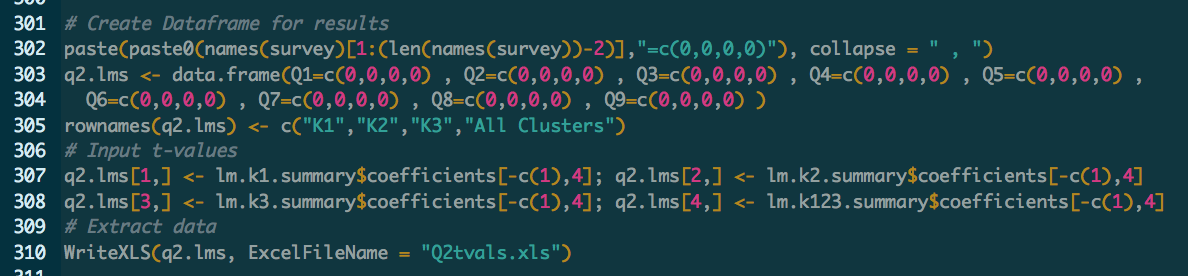
\includegraphics[width=16cm]{2b0.png}
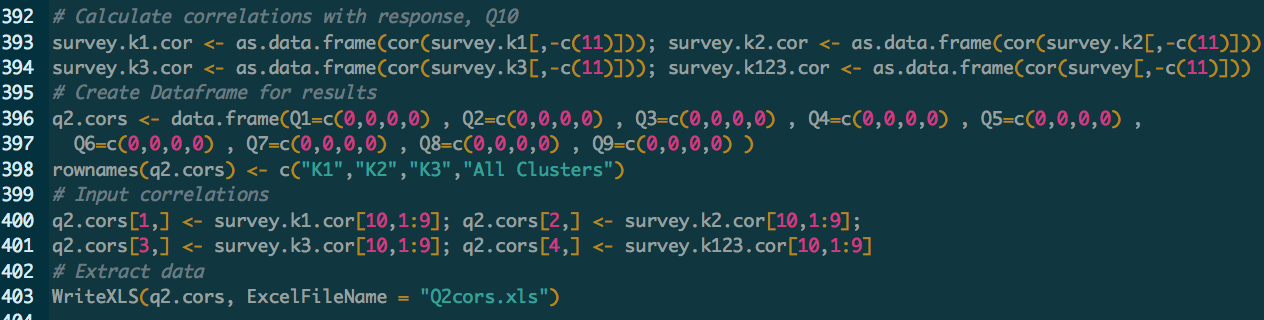
\includegraphics[width=16cm]{2b00.png}
\end{center}



%\begin{center}
%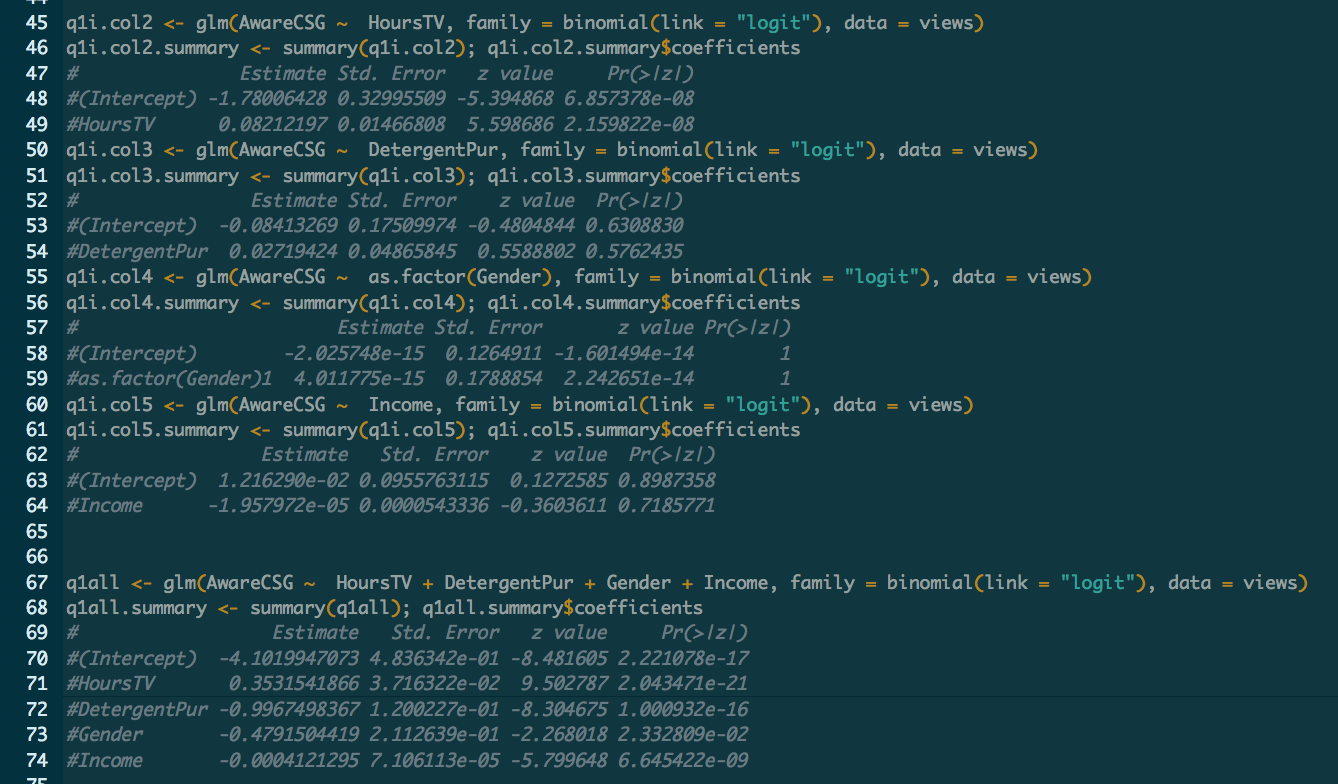
\includegraphics[width=16cm]{1a.png}
%\end{center}





\end{document}   
